\documentclass{article}
\usepackage{cmap}
\usepackage[utf8]{inputenc}
\usepackage[english,ukrainian]{babel}
\usepackage{graphicx}
\usepackage{geometry}
\usepackage{listings}
\usepackage{indentfirst}
\geometry{
	a4paper,
	left=20mm,
	right=20mm,
	top=20mm,
	bottom=20mm
}
\lstset{
	extendedchars=\true,
	tabsize=4,
	language=python,
	showstringspaces=false,
	showtabs=false,
	frame=lrtb,
	columns=fixed,
	keepspaces,
	breaklines=true
}
\graphicspath{ {pictures} }
\setlength{\parindent}{4em}
\newcommand\subject{Чисельні методи ПЗ}
\newcommand\lecturer{доцент кафедри ПЗ\\Мельник Н.Б.}
\newcommand\teacher{асистент кафедри ПЗ\\Гарматій Г.Ю.}
\newcommand\mygroup{ПЗ-16}
\newcommand\lab{1}
\newcommand\theme{Розв’язування нелінійних рівнянь методом дихотомії та методом хорд}
\newcommand\purpose{Ознайомлення на практиці з методами відокремлення дійсних ізольованих коренів нелінійних рівнянь. Вивчення методу дихотомії та методу хорд уточнення коренів}

\begin{document}
\begin{normalsize}
	\begin{titlepage}
		\thispagestyle{empty}
		\begin{center}
			\textbf{МІНІСТЕРСТВО ОСВІТИ І НАУКИ УКРАЇНИ\\
				НАЦІОНАЛЬНИЙ УНІВЕРСИТЕТ "ЛЬВІВСЬКА ПОЛІТЕХНІКА"}
		\end{center}
		\begin{flushright}
			Інститут \textbf{КНІТ}\\
			Кафедра \textbf{ПЗ}
		\end{flushright}
		\vspace{200pt}
		\begin{center}
			\textbf{ЗВІТ}\\
			\vspace{10pt}
			До лабораторної роботи № \lab\\
			\textbf{На тему}: “\textit{\theme}”\\
			\textbf{З дисципліни}: “\subject”
		\end{center}
		\vspace{112pt}
		\begin{flushright}
			
			\textbf{Лектор}:\\
			\lecturer\\
			\vspace{28pt}
			\textbf{Виконав}:\\
			
			студент групи \mygroup\\
			Коваленко Д.М.\\
			\vspace{28pt}
			\textbf{Прийняв}:\\
			
			\teacher\\
			
			\vspace{28pt}
			«\rule{1cm}{0.15mm}» \rule{1.5cm}{0.15mm} 2022 р.\\
			$\sum$ = \rule{1cm}{0.15mm}……………\\
			
		\end{flushright}
		\vspace{\fill}
		\begin{center}
			\textbf{Львів — 2022}
		\end{center}
	\end{titlepage}
		
	\begin{description}
		\item[Тема.] \theme.
		\item[Мета.] \purpose.
	\end{description}
	
	\section*{Індивідуальне завдання}

	\begin{enumerate}{}
		\item Ознайомитися з теоретичним матеріалом.
		\item Скласти програму розв’язування рівняння $x^3-6x^2-7=0$ методом дихотомії та методом хорд.
	\end{enumerate}
	
	\section*{Теоретичні відомості}
	
	Наступні методи розв’язування нелінійних рівнянь дозволяються знайти розв’язок для наступної задачі: Розглянемо рівняння $f(x) = 0$, у якому $f(x)$ є неперервною нелінійною функцією. На відрізку $[a, b]$ дана функція є монотонною та диференційованою, на ньому міститься єдиний корінь $x$ заданого рівняння, тобто $f(a)f(b) < 0$. Потрібно знайти значення кореня $x$ із заданою похибкою $\epsilon$.
	
	\subsection*{Метод поділу відрізка навпіл}
	
	Покладемо $a_0 = a$, $b_0 = b$ і обчислимо $x_0 = \frac{(a_0 + b_0)}{2}$. Якщо $f(x_0) = 0$, то $x = x_0$, у протилежному випадку, якщо $f(x_0) \neq 0$, то чинимо так: 
	\begin{list}{}{}
		\item $a_{n+1} = \{x_n$, якщо $sign f(a_n) = sign f(x_n)$\}, (1)
		\item $b_{n+1} = \{x_n$, якщо $sign f(b_n) = sign f(x_n)$\}, (2)
		\item $x_{n+1} = \frac{a_{n+1}+b_{n+1}}{2}$, $n = 1, 2, 3, ...$, (3)
	\end{list}
	і обчислюємо $f(x_{n+1})$. Якщо $f(x_{n+1}) = 0$, то ітераційний процес завершуємо і вважаємо, що $x \approx x_{n+1}$, а коли $f(x_{n+1}) \neq 0$, то продовжуємо ітераційний процес (1)-(3).
	
	\begin{figure}[h!]
		\centering
		\includegraphics[scale=0.4]{1}
		\caption{Геометрична інтерпретація методу дихотомії}
	\end{figure}

	\subsection*{Графічна інтерпретація методу поділу відрізку навпіл}
	
	Зі співвідношень (1), (2) видно, що $sign f(a_{n+1}) = sign f(a_{n})$ і $sign f(a_{n+1}) = sign f(a_{n})$. Тому $f(a_{n+1})f(b_{n+1})<0$, а отже шуканий корінь $x$ знаходиться на відрізку $[a_{n+1}, b_{n+1}]$. 
	
	Точність знаходиться за формулою $\epsilon = \frac{b-a}{2^{n+1}}$ тобто виконується нерівність $|x_n - x| \leq\frac{b-a}{2^{n+1}}$ (4).
	
	Звідси випливає, що кількість ітерацій. які необхідно провести для знаходження наближеного кореня рівняння $f(x) = 0$ з заданою точністю $\epsilon$ задовольняє співвідношенню $n = [log_2\frac{b-a}{\epsilon}-1]$, де $[\xi]$ - ціла частина числа $\xi$ (5)
	
	Серед переваг даного методу потрібно відзначити простоту реалізації та надійність. Недоліком наведеного методу є невелика швидкість його збіжності.
	
	\subsection*{Метод хорд}
	
	Суть методу хорд полягає в тому, що на відрізку $[a, b]$ малої довжини дугу функції $f(x)$ замінюють хордою $ab$ , яка її стягує. За наближене значення кореня приймають   абсцису точки перетину хорди з віссю $Ox$.
	
	Для довільного $(i + 1)$-го наближення точного значення кореня  $x$ для заданого рівняння використовують формулу $x_{i+1}=x_i-\frac{f(x_i)(b-x_i)}{f(b)-f(x_i)}$, $i = 1, 2, 3$..., де $x_0 = a$. (6)
	
	Дугу кривої стягують хордою доти, поки шуканий наближений корінь не досягне точності $\epsilon$, тобто $|x_{i+1}-x_i| < \epsilon$, (7)
	
	де $x_i$, $x_{i+1}$ - наближені значення кореня рівняння $f(x) = 0$, відповідно на $i$-му та $(i+1)$-му ітераційному кроці.
	
	\begin{figure}[h!]
		\centering
		\includegraphics[scale=0.7]{2}
		\hfill
		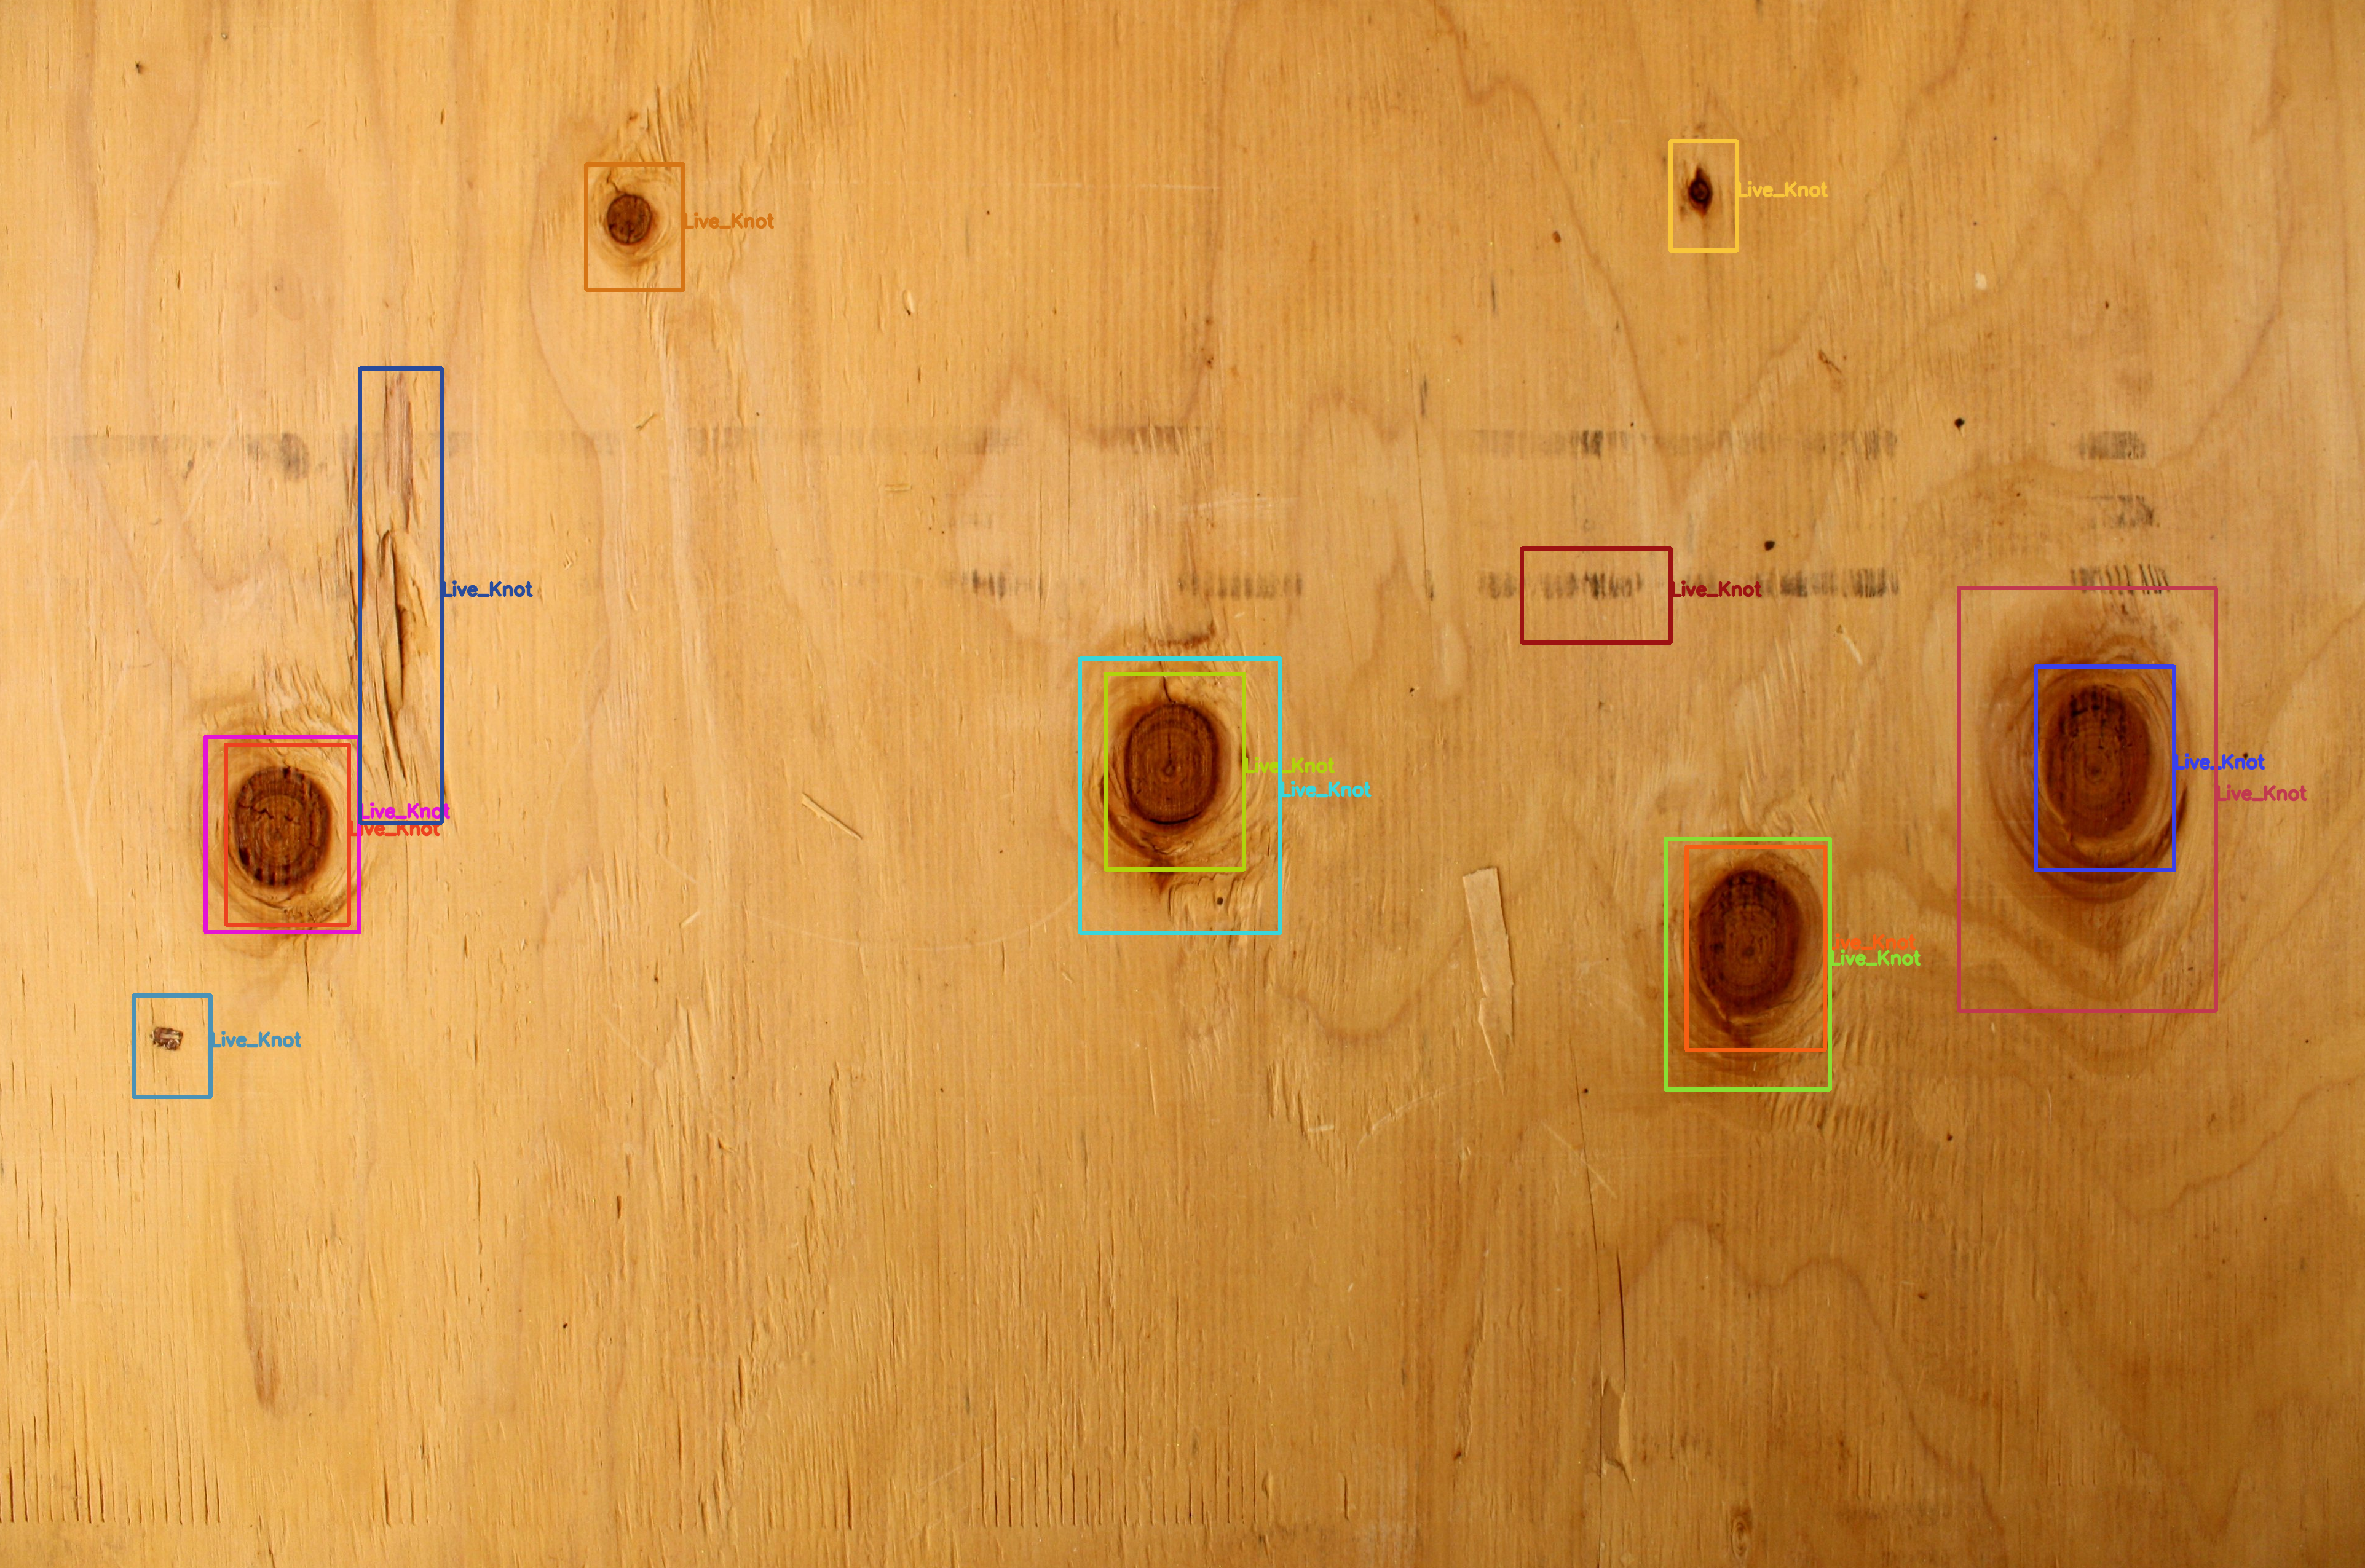
\includegraphics[scale=0.7]{3}
		\caption{Геометрична інтерпретація методу хорд}
	\end{figure}

	Для автоматизованого вибору рухомого кінця хорди і відповідно визначення співвідношення для обчислення наближеного значення кореня існує певне правило: нерухомим кінцем відрізка є той, для якого знак функції $f(x)$ співпадає зі знаком її другої похідної $f''(x)$. Якщо $f(b)f''(b) > 0$, то нерухомим є кінець $a(x_0 = b)$

	\section*{Хід роботи}
	\section*{Графічний метод}
	\begin{figure}[h!]
		\centering
		\includegraphics[scale=0.49]{4}
		\caption{Графічний метод}
	\end{figure}

	За графіком функції розв'язок даної функції розташований на відрізку $[6; 7]$.

	\section*{Аналітичний метод}
	Для аналітичного розв’язку визначимо монотонність функції f(x), для цього розв’яжемо рівняння $f'(x) = 0$ та знайдемо інтервали монотонності.
	
	$3x^2-12x=0$
	
	Інтервалами монотонності є $(-\infty; 0)$, $(0; 4)$, $(4; +\infty)$. Виберемо лише ті інтервали, де функція змінює знак $f(x) = f(x^3-6x^2-7) = +\infty$, $f(x) = f(x^3-6x^2-7) = -\infty$
	
	$f(4) < 0$, $f(+\infty) > 0$, Отже, $(4; +\infty)$ єдиний відрізок, де є корінь, бо на всіх інших знак не змінюється і функція є монотонною. Це значить, що корінь є і він лежить в цьому інтервалі. Знайдемо відрізок, де є корінь рівняння, для цього перевіримо знак функції у цілочисельних точках інтервалу.
	
	$f(6) = -7 < 0$ та $f(7) = 42 > 0$, отже корінь належить відрізку $[6; 7]$.
	
	\section*{Метод дихотомії}
	\textbf{\textit{Код програми}} (файл \textit{lab\_11.py}):
	\begin{lstlisting}
		
		class DichotomyMethod:
			""" Метод Дихотомії """
			
			
			def __init__(self, a, b, eps, f):
				self.a = a # Ліва межа
				self.b = b # Права межа
				self.x = 0 # Шуканий корінь
				self.eps = eps # Точність
				self.f = f # Функція
			
			
			def calculate(self):
				self.x = (self.a + self.b)/2
				print(f"a: {self.a}; b: {self.b}; x: {self.x}; f(x): 
					{self.calc_func(self.x, self.f)}")
				if abs(self.calc_func(self.x, self.f)) < self.eps: 
					return
				elif self.a == self.b: 
					return print("No roots")
				elif self.calc_func(self.a, self.f) * 
					self.calc_func(self.x, self.f) < 0:
					self.b = self.x
					return self.calculate()
				else:
					self.a = self.x
					return self.calculate()
			
			
			def calc_func(self, x, f):
				return eval(f.replace("x", str(x)))
		
		
		a = float(input("Введіть ліву межу: "))
		b = float(input("Введіть праву межу: "))
		eps = float(input("Введіть точність: "))
		f = input("Введіть функцію: ")
		
		d = DichotomyMethod(a, b, eps, f)
		d.calculate()
		
	\end{lstlisting}
	
	\begin{figure}[h!]
		\centering
		\includegraphics[scale=0.6]{6}
		\caption{Робота програми за допомогою методу дихотомії}
	\end{figure}
	
	\section*{Метод хорд}
	\textbf{\textit{Код програми}} (файл \textit{lab\_12.py}):
	\begin{lstlisting}		
		class SecantMethod:
			""" Метод Хорд """			
			
			def __init__(self, a, b, eps, f, f2):
				self.a = a # Ліва межа
				self.b = b # Права межа
				self.x = 0 # Шуканий корінь
				self.c = 0 # Нерухомий кінець
				self.eps = eps # Точність
				self.f = f # Функція
				self.f2 = f2 # Друга похідна функції
								
				if self.calc_func(self.a, self.f) * self.calc_func(self.a, self.f2) > 0:
					self.x = self.b
					self.c = self.a
				else:
					self.x = self.a
					self.c = self.b
						
			def calculate(self):
				print(f"c: {self.c}; x: {self.x}; f(x): 
					{self.calc_func(self.x, self.f)}")
				if abs(self.calc_func(self.x, self.f)) < self.eps: 
					return
				self.x = self.x - (self.calc_func(self.x, self.f) * (self.c - self.x)) 
					/ (self.calc_func(self.c, self.f) - self.calc_func(self.x, self.f))
				return self.calculate()
			
			def calc_func(self, x, f):
				return eval(f.replace("x", str(x)))
			
		a = float(input("Введіть ліву межу: "))
		b = float(input("Введіть праву межу: "))
		eps = float(input("Введіть точність: "))
		f = input("Введіть функцію: ")
		f2 = input("Введіть другу похідну функції: ")
		
		s = SecantMethod(a, b, eps, f, f2)
		s.calculate()
	\end{lstlisting}

	\begin{figure}[h!]
		\centering
		\includegraphics[scale=0.6]{7}
		\caption{Робота програми за допомогою методу хорд}
	\end{figure}

	\section*{Висновок}
	На лабораторній роботі я за допомогою хорд та дихотомії знайшов корені нелінійного рівняння $x^3-6x^2-7$ з точністю $0.001$, та розробив функції для розв’язку цих рівнянь.
	    
\end{normalsize}
\end{document}
